% Measuring What Eviction Costs: a methodology, and a bound for the clock sweep
% Build:  make   (needs texlive-publishers + cm-super; see Makefile)
\documentclass[sigconf,nonacm]{acmart}

\usepackage{booktabs}
\usepackage{multirow}
\usepackage{pgfplots}
\pgfplotsset{compat=1.17}
\usepackage{listings}
\usepackage{amsmath}

\lstset{
  basicstyle=\ttfamily\footnotesize,
  keywordstyle=\bfseries,
  commentstyle=\itshape,
  columns=fullflexible,
  frame=single,
  breaklines=true,
  language=C,
  morekeywords={uint64,bool,BufferDesc}
}

\begin{document}

\title{Measuring What Eviction Costs}
\subtitle{A methodology for page-replacement trade-offs, and a bound for the clock sweep}

\author{Greg Burd}
\affiliation{\institution{}\city{}\country{}}
\email{greg@burd.me}

\begin{abstract}
Page-replacement algorithms are evaluated almost exclusively on hit ratio.
That metric is blind to a failure mode we find in PostgreSQL's clock sweep: the
worst-case work of a \emph{single} buffer allocation equals the entire buffer
pool, measured to five significant figures at pool sizes from 4\,GiB to
96\,GiB, on two- and six-node NUMA hardware. One buffer read sweeps a million
descriptors. Hit ratio is unchanged while this happens, so no hit-ratio
benchmark can see it.

We propose evaluating an evictor on three axes instead of one---amplification
(advances per victim), the tail (worst advances for one allocation), and
replacement quality---and we show that the axes are independent enough that
optimising any one of them in isolation produces a wrong answer. Three results
make the case. First, replacing the 0..5 counter with a one-bit cooling state,
which we had previously proposed on grounds of simplicity, improves
amplification by $1.75\times$ and leaves the tail at $0.998$ of the pool: a
better constant, not a bound. Second, a termination rule that abandons
probation once it is observably unaffordable makes the tail $O(1)$---$34$
advances, constant across a $24\times$ range of pool sizes---and works equally
on the existing counter and on the one-bit state, so the bound and the state
encoding are orthogonal and separately adoptable. Third, the threshold that
rule needs is a direct dial between the two remaining axes: we measure the
entire curve, locate the knee, and show that a control loop adapting the
threshold is \emph{worse than a fixed value on both axes}, because the two
costs it trades are asymmetric in time.

The methodology is the contribution we expect to outlast the patch. An evictor
that is never asked what its worst allocation costs can hide an unbounded one.
\end{abstract}

\keywords{buffer management, page replacement, CLOCK, tail latency,
evaluation methodology, PostgreSQL}

\maketitle

\section{Introduction}

The literature on page replacement is a literature about hit ratio. From
CLOCK~\cite{corbato1968paging} through LRU-K~\cite{oneil1993lruk},
2Q~\cite{johnson1994lru2}, LIRS~\cite{jiang2002lirs},
ARC~\cite{megiddo2003arc}, CLOCK-Pro~\cite{jiang2005clockpro} and
S3-FIFO~\cite{yang2023s3fifo}, the question asked of a new algorithm is how
many misses it avoids, and the accepted way to answer is a trace replay or a
throughput benchmark. Cost of eviction appears, if at all, as a remark that the
algorithm is $O(1)$ amortised.

This paper is about what that framing misses. We examined PostgreSQL's clock
sweep, a CLOCK variant over a four-bit saturating counter, and found that a
single buffer allocation can perform work proportional to the entire buffer
pool---not occasionally, but reproducibly, at every pool size we tested, on
every topology we tried. Throughput and hit ratio are flat while it happens.
The pathology is invisible to the metric the field uses, and it is documented in
the source code's own comments, where it has sat unremarked for years because
nobody measured the quantity it describes.

Our argument is that an evictor should be characterised on three axes:

\begin{description}
\item[Amplification] clock advances per victim produced. This is the
  \emph{average} cost of eviction, and it is what a throughput benchmark
  indirectly samples.
\item[Tail] the largest number of advances any single allocation performs.
  This is the stall a user sees, and no average captures it.
\item[Replacement quality] hit ratio, measured where it matters---on the set
  the workload actually re-reads, not pool-wide.
\end{description}

The axes are not redundant. Each of our three results is a case where one axis
moves and another does not, in a way that would mislead anyone watching only
the conventional metric.

\paragraph{Contributions.}
\begin{enumerate}
\item A three-axis methodology for evaluating evictors, with the workload
  construction needed to exercise each axis (\S\ref{sec:method}), including the
  observation that the workload conventionally used to stress eviction is
  precisely the one that cannot reveal a tail.
\item A residency model (\S\ref{sec:model}) predicting candidate density
  $e^{-krT}$, and its empirical confirmation: PostgreSQL's worst-case
  allocation equals $N_{\text{buffers}}$ across a $24\times$ range
  (\S\ref{sec:tail}).
\item The negative result that a one-bit cooling state improves amplification
  and not the tail (\S\ref{sec:onebit}), which we report having previously
  argued for that change on the wrong grounds.
\item An $O(1)$ bound (\S\ref{sec:bound}) that is independent of the state
  encoding, demonstrated on both the stock counter and the one-bit state.
\item The full threshold trade-off curve (\S\ref{sec:theta}), and the negative
  result that an adaptive threshold is worse than a fixed one on both axes
  (\S\ref{sec:adaptive}), with the asymmetry argument that explains why.
\end{enumerate}

\section{The three axes, and how to measure them}
\label{sec:method}

\subsection{Why hit ratio alone is insufficient}

Consider two evictors that produce identical hit ratios and identical
throughput on a given workload. One finds a victim in a bounded number of
steps; the other, under the same workload, occasionally scans the entire pool
for one victim. These are not equivalent systems, and no hit-ratio measurement
distinguishes them. The distinguishing quantity---advances consumed by the
unluckiest allocation---is not conventionally reported.

We instrument it directly. Each arm of our comparison carries counters for
clock advances, victims produced, demotions performed, \emph{the maximum
advances consumed by any single allocation}, and forced claims. Amplification
is advances divided by victims; the tail is the running maximum.

\subsection{The workload that reveals a tail}

The conventional way to stress eviction is uniform random access over a working
set several times larger than the pool. We used exactly that for months and
measured nothing. It cannot work, and the reason is worth stating because it
generalises to any evaluation of this kind.

Under uniform access over a working set much larger than the pool, each
individual page has a vanishing access rate. No page is re-touched before the
clock hand returns to it, so every buffer decays to evictable and candidate
density stays near one. Such a workload measures eviction \emph{throughput};
it is structurally incapable of producing eviction \emph{starvation}.

Starvation requires the opposite configuration:

\begin{itemize}
\item a pool large enough that one pass takes real time;
\item a working set only \emph{slightly} larger than the pool, so most of the
  pool is warm rather than cold;
\item \emph{skewed} access, so individual pages are re-touched many times per
  pass;
\item enough concurrency that re-promotion races the hand.
\end{itemize}

Which is to say: the configuration of a large production database. We use a
table $1.15\times$ \texttt{shared\_buffers} and
\texttt{random\_zipfian}($s{=}1.10$).

\subsection{Measuring replacement quality where it matters}

Pool-wide hit ratio is also too coarse. A policy that evicts pages a workload
genuinely re-reads can still show a high pool-wide figure if most of the pool
is cold. To measure replacement quality we build a workload with an explicit
hot set---20\% of the pool, receiving 80\% of queries---alongside a cold stream
at $130\%$ of the pool that forces continuous eviction, and we report hit ratio
\emph{and resident page count for the hot relation specifically}. That is the
number probation exists to protect, and \S\ref{sec:theta} shows it moving when
pool-wide figures barely do.

\section{A residency model}
\label{sec:model}

Let $T$ be the time for the hand to complete one pass and model accesses to a
page as Poisson with rate $r$. For a counter of depth $k$ that saturates on
access, a buffer becomes evictable only after surviving $k$ consecutive passes
untouched, requiring an access-free interval of $kT$. Hence the steady-state
fraction of the pool that is evictable---the candidate density---is

\begin{equation}
\rho(k, r, T) \;\approx\; e^{-k r T},
\label{eq:density}
\end{equation}

and expected advances per victim is $1/\rho = e^{krT}$. Amplification is
exponential in the product of counter depth, access rate and pass time, and
since $T \propto N_{\text{buffers}}$, growing the pool grows the exponent.

\begin{figure}[t]
\centering
\begin{tikzpicture}
\begin{semilogyaxis}[
  width=\columnwidth, height=5cm,
  xlabel={$rT$ \quad (accesses per page per pass)},
  ylabel={candidate density $\rho$},
  xmin=0, xmax=4, ymin=1e-9, ymax=2,
  legend pos=south west, legend cell align=left,
  grid=both, grid style={gray!25},
]
\addplot[thick, mark=*, mark size=1.2pt] table[x index=0, y index=1] {data_density.dat};
\addlegendentry{$k=1$ (one-bit cooling)}
\addplot[thick, dashed, mark=square, mark size=1.2pt] table[x index=0, y index=2] {data_density.dat};
\addlegendentry{$k=5$ (PostgreSQL)}
\end{semilogyaxis}
\end{tikzpicture}
\caption{Candidate density falls exponentially in $rT$. Reducing counter depth
shifts the curve right by $5\times$ without changing its shape: both reach
arbitrarily low density, so no choice of $k$ yields a bound.}
\label{fig:density}
\end{figure}

Figure~\ref{fig:density} contains the paper's central structural claim. The
$k=5 \rightarrow k=1$ shift is real and large---at $rT=1$, candidate density
rises from $0.67\%$ to $37\%$, a factor of $55$---but it is only a shift. Both
curves go to zero, so for any $k$ there is a pool size at which density becomes
negligible. \emph{Changing the state encoding cannot bound the tail.} Only
changing the loop's termination rule can.

\section{Experimental setup}

\paragraph{Hardware.} \textbf{z1d.metal} (48 cores, 2 NUMA nodes, 384\,GiB,
data directory on RAID-0 local NVMe) and \textbf{r8i.metal-96xl} (384 cores, 6
NUMA nodes, 3\,TiB). Huge pages on, transparent huge pages off, NUMA balancing
off, postmaster interleaved.

\paragraph{Arms.} Five builds of PostgreSQL 20devel,
\texttt{debugoptimized}, assertions off, differing \emph{only} in the eviction
path: \textsc{master} (0..5 counter); \textsc{+claim} (the bound of
\S\ref{sec:bound} applied to that counter, \emph{no other change});
\textsc{1-bit} (cooling state); \textsc{1-bit+claim}; and
\textsc{1-bit+claim+bgw} (background staging). All five carry the identical
instrument. Three runs per point; counters sampled after a 60\,s warmup and
differenced.

\section{The tail is the whole pool}
\label{sec:tail}

\begin{table}[t]
\centering
\caption{The three axes across five arms. $\max$ ticks is the largest number of
clock advances performed by any single allocation.}
\label{tab:arms}
\small
\begin{tabular}{llrrrr}
\toprule
$s_b$ & arm & ampl. & $\max$ ticks & $\max/N_{\text{buf}}$ & hit \% \\
\midrule
\multirow{5}{*}{8\,GiB}
 & master         & 5.87 & 1{,}048{,}614 & \textbf{1.0000} & 99.706 \\
 & +claim         & 5.25 & \textbf{34}   & 0.00003 & 99.691 \\
 & 1-bit          & 3.34 & 1{,}046{,}554 & \textbf{0.9981} & 99.707 \\
 & 1-bit+claim    & 3.39 & \textbf{35}   & 0.00003 & 99.707 \\
 & 1-bit+claim+bgw& 3.11 & \textbf{34}   & 0.00003 & 99.684 \\
\midrule
\multirow{5}{*}{32\,GiB}
 & master         & 2.11 & 4{,}194{,}342 & \textbf{1.0000} & 99.564 \\
 & +claim         & 4.26 & \textbf{34}   & 0.00001 & 99.591 \\
 & 1-bit          & 1.32 & 4{,}192{,}282 & \textbf{0.9995} & 99.618 \\
 & 1-bit+claim    & 1.32 & \textbf{34}   & 0.00001 & 99.617 \\
 & 1-bit+claim+bgw& 1.32 & \textbf{33}   & 0.00001 & 99.617 \\
\midrule
96\,GiB & master  & 1.17 & 12{,}582{,}950 & \textbf{1.0000} & 99.410 \\
\bottomrule
\end{tabular}
\end{table}

Table~\ref{tab:arms} is the paper in one place. Read the
$\max/N_{\text{buffers}}$ column for \textsc{master}: it is $1.0000$ at every
pool size. At 4\,GiB the pool holds $524{,}288$ buffers and the worst
allocation consumed $524{,}326$ advances; at 96\,GiB, $12{,}582{,}912$ buffers
and $12{,}582{,}950$ advances. The excess is $38$ advances in both
cases---one cache line of descriptors---so the behaviour is exactly one full
pass plus a small constant, across a $24\times$ range of pool sizes.

Throughput is flat across all five arms at every point, within $2\%$ and with
overlapping run-to-run ranges, and pool-wide hit ratio moves by hundredths of a
point. An evaluation on the conventional axes would conclude that these five
systems are the same system.

The result is independent of NUMA topology: \textsc{master} pins to the
\emph{same} maximum on two nodes and on six, while throughput between those
machines differs by $1.6\times$. The pathology belongs to the replacement
algorithm, not to memory placement, and NUMA-partitioning
work~\cite{vondra_numa} will not address it---partitioning reduces $T$ per
partition but leaves the exponential intact within each.

\section{Fewer states is a better constant, not a bound}
\label{sec:onebit}

We previously proposed replacing \texttt{usage\_count} with a one-bit cooling
state in the manner of LeanStore~\cite{leanstore2018}, arguing it on
simplicity---two states and no magic constant instead of six states and a
tunable five---and measuring its throughput effect as nil.

Table~\ref{tab:arms} shows what the change does on the three axes.
Amplification improves consistently, $5.87 \rightarrow 3.34$ at 8\,GiB and
$2.11 \rightarrow 1.32$ at 32\,GiB, which is Equation~\ref{eq:density} behaving
as predicted when $k$ falls from five to one. The tail does not move: $0.9981$
and $0.9995$ of the pool, still a full pass, still
$O(N_{\text{buffers}})$. A page re-promoted within $T$ is immortal whether
promotion sets a counter to five or a bit to one.

We report this as a negative result against our own earlier proposal. The state
encoding was never what made allocations unbounded, and an argument from
simplicity could not have discovered that, because simplicity is not one of the
three axes.

\section{A bound from evidence}
\label{sec:bound}

The loop's defect is that it treats decrementing as progress without limit. It
will decrement forever, because each decrement is locally a step toward a
victim even when the workload is globally restoring them faster.

Probation exists so a buffer gets passes of grace in which a new access can
rescue it. That is a good default, affordable only while victims can still be
found. Once a single call has decremented $\Theta$ buffers without encountering
one at zero, the pool is \emph{observably} hotter than the hand can
traverse---a direct measurement of the quantity that matters, not a heuristic
on a proxy---and the sweep claims the next unpinned buffer:

\begin{lstlisting}
if (BUF_STATE_GET_USAGECOUNT(state) != 0) {
  if (decremented < BUF_DECREMENT_CLAIM_THRESHOLD) {
    state -= BUF_USAGECOUNT_ONE;
    if (CAS(&buf->state, state)) {
      decremented++;
      trycounter = NBuffers;
      break;
    }
    continue;
  }
  /* pressure: claim it. usage_count is cleared when the
   * victim is reused, so no need to reach zero first. */
  pg_atomic_fetch_add_u64(&ctl->numForcedClaims, 1);
}
state += BUF_REFCOUNT_ONE;      /* claim */
\end{lstlisting}

The counter is call-local, so the common path takes no additional atomic; and
under any workload the hand keeps up with, $\Theta$ is never reached and the
code path is identical to before.

\paragraph{The bound is independent of the state encoding.} This is the
practically important finding. Table~\ref{tab:arms}'s \textsc{+claim} row is
this rule applied to the \emph{unmodified} 0..5 counter---no cooling state, no
change to any buffer state bit, no change to the background writer or the ring
buffers---and its tail is $34$, the same as the one-bit arm's $35$. Amplification
stays at the stock arm's level ($5.25$ versus $5.87$), as it must: the rule
fires only in the tail, so it should not move the mean.

The bound and the encoding are therefore separately adoptable. An implementer
who wants bounded allocations need not accept a new replacement policy, and the
patch that delivers the bound touches two files.

\section{The threshold is a dial, and we measured it}
\label{sec:theta}

$\Theta$ trades the two remaining axes against each other. Rather than defend a
constant, we measured the whole curve, sweeping $\Theta$ over three decades at
runtime ($\Theta=0$ meaning never claim, i.e.\ stock).

\begin{table}[t]
\centering
\caption{Threshold sensitivity, and its cost measured on a hot set that
probation exists to protect (20\% of pool, 80\% of queries, with a cold stream
at $130\%$ of pool forcing eviction).}
\label{tab:theta}
\small
\begin{tabular}{rrrrrr}
\toprule
$\Theta$ & $\max$ ticks & ampl. & claims & hot hit \% & hot pages evicted \\
\midrule
1        & 3      & 2.00 & 825{,}450 & --- & --- \\
4        & 6      & 4.06 & 400{,}090 & 98.2313 & 4{,}519 \\
16       & 18     & 5.92 & 59{,}652  & --- & --- \\
32       & 36     & 5.37 & 5{,}576   & 99.9671 & 11 \\
128      & 130    & 5.19 & 64        & 99.9998 & \textbf{0} \\
1024     & 1{,}026& 5.14 & 0         & --- & --- \\
0 (none) & 61{,}532 & 5.11 & 0       & 100.0000 & 0 \\
\bottomrule
\end{tabular}
\end{table}

\begin{figure}[t]
\centering
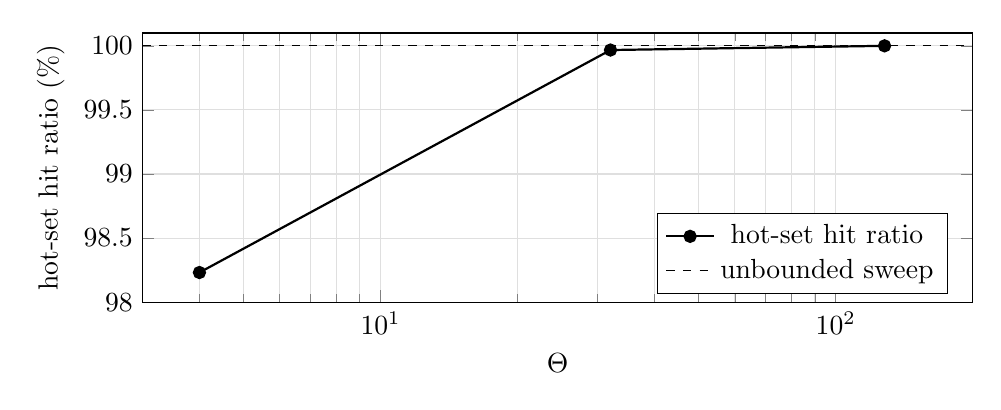
\begin{tikzpicture}
\begin{semilogxaxis}[
  width=\columnwidth, height=5cm,
  xlabel={$\Theta$}, ylabel={hot-set hit ratio (\%)},
  xmin=3, xmax=200, ymin=98, ymax=100.1,
  grid=both, grid style={gray!25},
  legend pos=south east,
]
\addplot[thick, mark=*] coordinates {(4,98.2313) (32,99.9671) (128,99.9998)};
\addlegendentry{hot-set hit ratio}
\addplot[dashed, domain=3:200, samples=2] {100};
\addlegendentry{unbounded sweep}
\end{semilogxaxis}
\end{tikzpicture}
\caption{Replacement quality against threshold. Below $\Theta\approx32$ the
claim path evicts pages the workload is actively re-reading; by $\Theta=128$ it
evicts none and hit ratio equals an unbounded sweep's.}
\label{fig:harm}
\end{figure}

Two readings. First, $\max \text{ticks} \approx \Theta + 2$ across three
decades, so $\Theta$ is a direct and predictable dial on the tail rather than
an opaque heuristic. Second, the cost of claiming is real and now
quantified---this closes a question we previously had to leave open. On the
hot-set workload, $\Theta=4$ evicts $4{,}519$ genuinely hot pages and costs
$1.77$ points of hot-set hit ratio; $\Theta=32$ evicts eleven and costs
$0.03$; $\Theta=128$ evicts none and costs nothing measurable, while still
bounding the tail at $130$ advances against an unbounded scan's $10^6$.

$\Theta=128$ is therefore the defensible default: four orders of magnitude of
tail reduction for no measurable loss of replacement quality. Note that
pool-wide hit ratio would have hidden this---it moves by $0.65$ points where
the hot set moves by $1.77$---which is the methodological point of
\S\ref{sec:method}.3 made concrete.

\section{Why adapting the threshold is worse}
\label{sec:adaptive}

A fixed $\Theta$ picks one point on Table~\ref{tab:theta} and keeps paying for
it, so adapting it is the obvious next idea, and we implemented it: each
backend starts at $\Theta_{\max}=1024$ (no claims, behaviour identical to an
unbounded sweep), halves on each forced claim, and recovers by one on each
claim-free allocation. Additive-increase/multiplicative-decrease, backend-local,
no shared state.

It is worse than a fixed threshold on both axes.

\begin{table}[h]
\centering
\caption{Adaptive versus fixed, same workload, alternated.}
\label{tab:adaptive}
\small
\begin{tabular}{lrrrr}
\toprule
variant & $\max$ ticks & claims & hit \% & ampl. \\
\midrule
unbounded      & 57{,}908 & 0        & 99.7083 & 5.02 \\
fixed $\Theta{=}32$ & \textbf{34} & 7{,}702 & \textbf{99.7023} & 5.41 \\
adaptive (AIMD)& 1{,}025  & 188{,}962 & 99.6675 & 5.60 \\
\bottomrule
\end{tabular}
\end{table}

The controller oscillates rather than converging. At roughly $600$k
allocations per second, recovery at $+1$ per claim-free allocation returns
$\Theta$ from the floor to $\Theta_{\max}$ in milliseconds, and claim-free
allocations vastly outnumber claims. So the loop sits near $\Theta_{\max}$
almost always---paying a full $1024$-advance scan on each starvation
event---while re-entering back-off often enough to claim $25\times$ more than
the fixed threshold does. Worst of both axes.

The deeper reason is the asymmetry we had the data to see and did not use.
Hit-ratio loss is incurred on \emph{every} claim, continuously; the unbounded
scan is incurred only by the rare allocation that starves. A controller whose
recovery is fast relative to the arrival rate of starvation events cannot
exploit that asymmetry, and the measured curve already saturates: hit ratio at
$\Theta=128$ equals the unbounded sweep's, so there is nothing above $128$ for
an adaptive scheme to win. The engineering answer is a fixed threshold at the
knee, and the control loop is complexity with a failure mode and no measured
benefit.

We report this because it closes an open question in the direction opposite to
the one we expected, and because ``make it adaptive'' is the reflex suggestion
for any constant.

\section{Threats to validity}

Our evidence that this pathology costs production users is second-hand: reports
of multi-second stalls on large instances, consistent with the mechanism but
not instrumented by us. The cheapest confirmation requires no patch---if
\texttt{pg\_buffercache\_usage\_counts()} shows a pool piled at
\texttt{usage\_count}~5 with little at~0, the sweep has no candidates and every
allocation is paying to search.

Pool sizes reach 96\,GiB where production instances reach terabytes, and $T$
grows with the pool, so we expect our figures to understate the effect. The
hot-set workload is one construction; others may locate the knee differently,
though the shape should follow Equation~\ref{eq:density}. The AIMD result
falsifies one adaptive scheme, not every possible one---a controller with
hysteresis on the order of the starvation inter-arrival time remains untested,
and we doubt it is worth the complexity given the saturation at $\Theta=128$.
All measurements are single-instance; replication and recovery are unexamined.

\section{Conclusion}

PostgreSQL's clock sweep has an unbounded worst case, and it is not missing the
bound by a little: a single allocation sweeps the entire pool, reproducibly, at
every size we measured, on both topologies we tried, while throughput and hit
ratio sit still. The code's own comments have described the possibility for
years; what was missing was anyone measuring the quantity they describe.

The appealing fix---a cleaner state encoding, one bit instead of six---improves
the average by $1.75\times$ and leaves the worst case at $0.998$ of the pool.
We know because we proposed it first. Bounding the tail requires changing what
the loop accepts as progress, and that change is independent of the encoding:
applied to the unmodified counter it gives the same $O(1)$ bound in two files.
Its one constant is a dial we measured end to end, with a knee at $128$ where
four orders of magnitude of tail reduction cost no measurable replacement
quality, and an adaptive version of that dial is measurably worse than leaving
it fixed.

What we would most like to see adopted is the methodology. Each of the three
results above is a case where the conventional metric is silent: hit ratio
cannot see an unbounded allocation, throughput cannot see it either, and the
pool-wide hit ratio that would judge the fix understates its cost by a factor
of three compared to measuring the set the workload actually re-reads. An
evictor that is never asked what its worst allocation costs can hide one that
costs everything.

\bibliographystyle{ACM-Reference-Format}
\bibliography{refs}

\end{document}
